Generalized symbols\ldots{}

Geometron is a geometric meta-langauge. That is it is a language for
building geometric languages, which is itself expressed entirely through
geometry. The three main components of Geometron are the ``Geometron
Virtual Machine'', or GVM, the Geometron Hypercube, and the Cursor.

The cursor is like a ``turtle'' in other geometry languages such as
\href{https://en.wikipedia.org/wiki/Logo_(programming_language)}{Logo},
it is a collection of global geometric variable which can be acted on.
These global variables might be the position of a cursor in an xy plane,
of a cube in an xyz space, of a physical robot tool, or of any
technology with geometry in it. The geometric actions discussed below
are on this abstraction, which can also be thought as a ``tool'', which
in some cases it literally is. However ``tool'' can be misleading since
the state of the cursor is not simply a position but can include
variables like ``step size'' which are abstract and not embodied in the
physical state of a physical tool.

The GVM is an abstract ``machine'' of pure thought which carries out
geometric actions. The actions of the GVM are arranged geometrically
into two cubes (hence ``hypercube'') each composed of 8x8x8 cells. Each
of these 512 cells has an address based on its geometric location. All
addresses start with the number ``0'', and indexes count up from 0
rather than 1. One cube has addresses from 0 through 0777, and the other
has addresses from 01000 through 01777. Each cell in the Hypercube
represents either a geometric action or a list of addresses in the
hypercube which the GVM will execute in order. The GVM is fed a
``glyph'' which is a sequence of Hypercube addresses, and it executes
the actions in the glyph in order. Some actions are therefore themselves
glyphs, which in turn can be composed of sub-glyphs and so on. Infinite
loops can easily be created this way.

The zero cube from 0 through 0777 is the ``Action Cube'', which
represents actions themselves we wish to use the GVM for. Each action
has a corresponding symbol in the symbol cube or 1 cube from 01000
through 01777, which is a glyph designed to communicate the meaning of
the action to a human user.

The Action Cube is divided into layers, which organize the types of
information into different categories.

0-07: left open for future use.

010-037: ``root magic'', or actions which act on the Hypercube itself or
the document being used to interact with Geometron.

040-0176: Printable ASCII. These are used to either place a ASCII
character on the Word Stack (to be printed using the action at 0365) or
to identify the action taken when a key is struck on a keyboard
connected to a GVM

0177: do nothing

0200-0217: Fixed shapes, glyphs composed of sequences of actions which
are left alone for general use, not edited frequently

0220-0277: General shapes. Glyphs used to create geometric languages
such as schematic symbols, graph theory arrows, cross stitch patterns,
flow charts etc.

0300-0377: Primary two dimensional geometric actions used on computer
screens. These are further broken down into the Action Tablet documented
below.

0400-0477: Machine actions. These include manipulation of global machine
variables such as step size or speed of movement. They will generally be
machine specific although we will document the specific values for the
Token Printer below. IN actual Arduino code these are generally mapped
to ASCII, as is the set below.

0500-0577: Shapes made up of sequences of actions in the 0400-0477
space. These can also include the entire rest of the Hypercube, and
allow for a combination of 2d, 3d, and mechanical actions, so that for
instance a cutting tool path can be saved as a 2d image in addition to
the direct control of the machine using Arduino.

0600-0677: Shapes made up of sequences of actions in the 0700-0777
space. These can be used to build whole complex languages of three
dimensional shapes for 3d printing design as well as VR and AR.

0700-0777: 3d actions. These actions are used to construct three
dimensional abstract geometry. Specifically in the Trash Robot Geometron
system they are used to build .x3d and .stl files which can be used for
VR and 3d printing respectively. Learn more from
\href{scrolls/geometron3d}{3d scroll}. Or just try out the system on
\url{voxel.html}.

This arrangement then maps to symbols which have meaning to humans
pointing to the actions. Note that for the ASCII values this maps to a
font of the printable ASCII, which can be in any human language.
Building more complex human languages like the CJK characters or fractal
Arabic calligraphy, we can add whole cubes to the Hypercube. The range
of characters between 01040 and 01176 are called a ``font''.

The software presented here allows us to use Geometron to make computer
files in either the vector graphics .svg format or the bitmap format
.png of all sizes, styles and shapes, save them, edit them, replicate
and share them. These can be used as icons, as symbols in Maps, as
figures in Scrolls, as art, or as patterns which can be directly
transferred to a laser cutter to create all the laser cut acrylic shapes
which are used for the arts and crafts projects presented in this work.

In addition, the software presented here uses the same Hypercube and GVM
to create, edit, and replicate 3d files which are saved in .stl for 3d
printing or x3d for VR and AR or games.

Perhaps most importantly, however, the software presented here allows us
to create generalized symbols using Geometron which use physical
machines to make physical matter with the symbols we create in
Geometron. Extending the system to more cubes in higher address spaces
can allow for a totally generalized methodology for creating geometric
languages for any kind of fabrication, media, display or design
technology.

Symbols are created using \url{symbol.html}. One edits a glyph which is
displayed in a canvas element on the screen by either hitting keys which
correspond to actions or soft keys on the screen. Another canvas element
displays the sequence of symbols corresponding to the actions in the
glyph. The arrow and delete keys are used for editing by keyboard, and
there are equivalent symbols on the soft key menu.

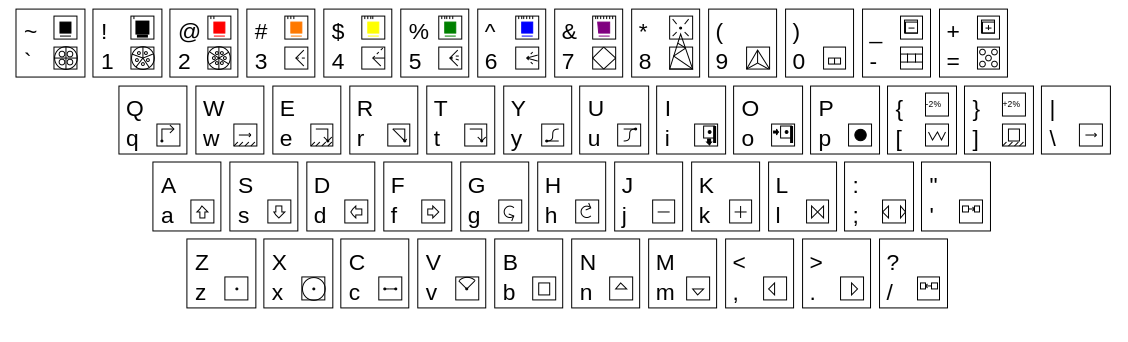
\includegraphics{iconsymbols/keyboard.svg}

Glyphs are stored in software as strings formed from sequences of
numbers separated by commas. As you edit a glyph the string will change
in an input. That string can be copied to the clip board and saved,
emailed or text messaged to someone who can paste it in their own
Geometron software to copy the symbol.

Actions of symbol.html

\includegraphics{iconsymbols/actiontablet.svg}

\href{scrolls/hellogeometron}{Learn to operate Geometron with the Hello
Geometron Scroll}

\href{https://lafelabs.github.io/book_of_geometron.html}{read a book ish
document of an obsolete version of Geometron in the Book of Geometron
here}

\hypertarget{geometron}{%
\section{Geometron}\label{geometron}}

The purpose of science and technology is maximize the ability of the
human mind to interact with our physical environment. As our society
becomes increasingly technological, we find that our power in that
society is based on our ability to control machines. As machines become
increasingly complex, the groups of people able to control them become
more and more specialized, and most people lose more and more control
with each new more complex generation of machines. In this work we seek
to push back against this trend by building a language for the natural
control of machines by people. The intent here is to build not just a
language but a linguistic framework which can be used in many context on
many technologies for \emph{all} people to wield more control over
\emph{all} machines. By gearing the operation of the language directly
toward industrial automation machines it is our intent to build a
pathway for ordinary people across Humanity to have direct control of
the means of industrial production at the local level.

Geometron is a language for humans to control machines using the natural
structure of both machine operation and the human mind. We consider
three structures to be fundamental to how our minds organize thought
which are mirrored in machine operation. Those are:

\begin{enumerate}
\def\labelenumi{\arabic{enumi}.}
\item
  Cataloging or listing of things. One of the most basic things we do
  when we organize information is make lists of things: the periodic
  table of elements, the alphabet, the organization of the base 10
  number system, division of light into discrete colors, the system of
  organizing mailing addresses etc. This is a structure mirrored in how
  modern computers are constructed: information is stored based on an
  addresses. Addresses in a modern computer also often contain other
  addresses, direction the operation of the machine from one point in
  memory to another. While arbitrarily complex and varied types of
  information can be stored at a memory address, it is useful in both
  machine architecture and human language to impose a structure which is
  universal across many specific elements. For instance, the mailing
  address format can point to a vast estate, a PO box, an individual, a
  corporation, etc. but it's useful to have all these under the one
  unified system of addressing. Another example of this is library call
  numbers, which map all of human knowledge to a simple string of
  numbers and letters.
\item
  Naming of things. Perhaps the most fundamental form of abstract human
  language is using a word to point to a thing. In particular the
  ability of the human mind to chain the naming process together is
  fundamental to human thought. For example, we use names to point to
  people, but also use the word ``person'' to point to each individual
  person. That is, words are used to point from any kind of thing to any
  other kind of thing. The naming process creates complex networks of
  relations between things which we use to build up our whole view of
  the world. As with the cataloging process, this function is mirrored
  in the architecture of our machines. The languages we use to program
  machines are constantly using pieces of information, called variables,
  which represent some meaning separate from the name of that
  information. For instance, in commonly used web software to have
  something called a ``shopping cart'' which is an abstract thing
  pointing to a list of things a person plans to buy. In addition to
  information technology we consider the mappings which take place in
  machines where something like a pull on a steering wheel can map to a
  whole sequence of things, from a computer to power steering, to the
  many machines which respond in concert to such actions. This is not
  exactly naming, but has a similar structure, where things are mapped
  to other things.
\item
  Geometry. In this work we assume that certain types of geometry are
  fundamental to the structure of both human thought and to how all
  machines we build operate. Most of the structure of the language
  presented here is based on either considering geometry which feels
  natural to the human mind like ``left'' and ``right'' and geometry
  natural to the operation of a machine like ``distance between plants''
  in an agricultural robot or distance between pixels in a display.
\end{enumerate}

The Geometron language uses all three of these elements to construct a
geometric meta-language: a language for building languages. The language
consists of geometric \emph{actions} organized according to an
addressing system called the Geometron Hypercube. Each action is
represented by a symbol which is itself drawn using the actions of
Geometron.

In order to build a language that is as natural as possible for people
to understand we begin with what geometry we all consider natural and
work from there to a specific implementation. The most basic geometric
action we consider are movement by one unit in the basic directions
``forward'', ``backward'', ``left'' and ``right''. These words in human
language have meanings which depend on context, and that is how they
work in Geometron as well. ``Go forward'' is a universal message which
can be expressed in any human language, and yet its precise meaning
depends on several unspoken assumptions. There is an implied
direction-state of the speaker or listener. There is also an implied
angle from which ``left'' and ``right'' deviate from ``forward'', and an
implied unit which one might move. For example if giving driving
directions in a city on a grid, we might say ``drive 10 blocks forward
along the street you're on, turn right, and go 5 blocks, then left and
one more block''. By abstracting this language we can generalize to
something like ``10 units forward, 5 units right, 1 unit forward'' and
this can apply to paces walked, pixels on a screen, or trees in an
orchard. That is, the idea of a grid of points which we navigate with
simple lefts, rights, forwards, and backs, is a \emph{universal} idea,
which does not depend on special technical knowledge, but which we can
expect anyone to understand even without written or technical language.
All this also implies that there is a position of the listener/speaker
who is depicting this sequence of actions.

To summarize the previous paragraph, we pose that there is a geometric
``state'' which all humans understand how to manipulate. This state
consists of position, orientation, a basic unit like ``blocks'',
``feet'', ``steps'', ``football fields'' etc, and an implied angle by
which we turn (usually 90 degrees unless specified otherwise). We can
then create symbols to represent the basic operations of movement of
this state as follows:

\begin{itemize}
\tightlist
\item
  go forward 1 unit
\item
  go back 1 unit
\item
  go left 1 unit
\item
  go right 1 unit
\item
  rotate left
\item
  rotate right
\end{itemize}

We construct symbols for these which get as close as possible to using a
universal language which all people will recognize, in this case arrows.
These symbols are then:

\includegraphics{iconsymbols/movement-symbols.svg}

These symbols are intended to be as universal as possible, avoiding both
the selection of a language like English to draw from as well as
machine-specific or technical mathematical language. Each of these
symbols is itself made up of geometric actions which will be documented
below: changing of scales, rotations by various angles, and natural
geometric constructions such as circles, arcs, line segments, and paths
of joined segments. We immediately see the power of building a language
for creating symbols which is written in itself. Just as human languages
contain dictionaries consisting entirely of definitions written in the
language being documented, we can create a language of geometric actions
built entirely of symbols using those actions.

This is the most fundamental power of the Geometron language: to make
arbitrary symbols which can then be used to program all sorts of other
more general machine operations. Once we have the ability to make
arbitrary symbols, we can immediately use those to construct commands
for operating any machine. For example, if we have a simple robot that
simply consists of a stage that can be moved in two directions with a
tool over the top of it, we can label one with a red arrow and one with
a green arrow, select some basic movement unit, say 1/100th of the total
span of the stage, and start writing programs by using a sequence of
these arrow-motion actions. In this language, a program that moves left
on the red direction, then out in the green direction and back might
look like this:

\includegraphics{robot-movements-symbols.svg}

This simple concept can be very powerful when combined with direct
controls of a machine. A user who starts moving labelled levers to
control a machine can immediately enter a sequence of actions based on
the experience of operating that machine to automate a process. This is
the level at which automation can be truly controlled by the people of
the world, and is a necessary condition for people to ever control their
own means of automation.

With the goal in mind of being able to build a universal symbolic
language for controlling machines, we may now proceed to documenting how
that language is constructed. To reference the introduction here, there
are three tools we will use: assigning addresses to things, assigning
symbols to actions (in essence a naming of things), and the use of
universal geometry of Nature. When we speak of ``actions'' in Geometron
it is useful to have some sort of object which is carrying out those
actions. That object is called the ``Geometron Virtual Machine'', or
GVM. Depending on context, the GVM might draw on a computer screen,
control a robot, create 3d structures, control the function of buttons
and keys, encode writing in human languages and edit the structure of
Geoemtron itself. In all cases, each action has a symbol, which is
itself just a sequence of actions. Each action has an address which is
made up of three numbers, each of which can range from 0 to 7. Types of
action are organized by the first of the three numbers (e.g.~machine
movements vs.~2d geometry vs.~3d actions etc.). This system divides
actions up into tablets which have an 8x8 array of ``boxes'' each of
which maps to some kind of geometric action. The 8x8 array is an
aesthetically pleasing way to organize information which pushes the
bounds of what is comprehensible to look at for a person while also
fitting the convenience of using powers of two for interaction with
computers.

Each action address is matched by a symbol address which adds a ``1'' to
the left of the address. All addresses start with a ``0'' to indicate
the format as a Geometron address, and to indicate for computer code
that this is a base 8 system. Thus for example if the action for ``draw
a circle'' is at address 0341, the address 01341 will contain the
sequence of actions which draws the symbol representing the drawing of a
circle. This ability of Geometron to pivot meaning radically based on
context mirrors the power of human language in contrast to most computer
languages.

The structure of addresses has its own geometry. A stack of 8 tablets,
each represented as an 8x8 array makes an 8x8x8 cube. We have two of
these cubes, the ``action cube'' and the ``symbol cube''. Again while
this might seem cumbersome and one can get lost in the details of the
exact functions of addresses, this is intended to create large scale
structures which anyone can understand: every action is a location in
one of two cubes of 8x8x8 cells. Ever action in the symbol cube consists
of a sequence of actions which create the symbol representing the
matching action in the action cube. That is, each cell in the 8x8x8
symbol cube contains a sequence of addresses in the action cube.

The action cube is divided into different types of function. At this
point the need to give the language enough specificity to actually
function requires that we dive in in some depth to the exact functions
used. The address ranges in the Action Cube are as follows:

\begin{itemize}
\tightlist
\item
  00-037: Actions on the functioning of Geometron itself, such as moving
  a cursor, deleting a symbol, or clearing a symbol. Taken together
  these types of action are called ``root magic''.
\item
  040-0176: ASCII. These numbers correspond to the printable characters
  standard on computers in the English speaking world. ASCII stands for
  ``American Standard Code for Information Interchange'' and is a
  universally recognized way to encode English characters on computers.
  The contents of these addresses are used to map key functions on a
  keyboard to anything in the Geometron Hypercube. For instance the
  address representing the letter lowercase `a' is 0141, and in the
  default configuration that contains the address for ``move forward by
  one unit'', which is 0330. So when a user strikes the `a' key, that
  adds the action ``move forward one unit'' to the sequence being
  edited. The symbols corresponding to these locations in the Action
  Cube are then symbols of the printable characters, which represent a
  font. That is, for example, the address in the Symbol Cube
  corresponding to the lowercase letter `a' is 01141. In the address
  01141 in the Symbol cube we will find a sequence of actions describing
  how to draw a lowercase letter `a'. This creates an immediate way to
  handle all human languages and keyboard mappings, as we can simply
  edit the contents of the Geometron Hypercube to both change key
  functions and change all the printable characters in a set of 95 from
  space bar to tilde.
\item
  0177: do nothing
\item
  0200-0277: Shapes. Each of these addresses contains a sequence of
  actions. That is, rather than computer code directly doing something,
  when one of these actions is triggered, it maps to a sequence of
  actions stored at that address. This can lead to infinite recursive
  loops, and it is useful to add functions that break infinite loops or
  avoid them. Formally, the sequences in this range can reference any
  address in the whole hypercube but by \emph{convention} they are taken
  to generally be two dimensional constructions out of which symbols are
  constructed.\\
\item
  0300-0377: Symbol action geometry. This is the heart of what makes the
  whole system work. These are the actions which are used to create
  symbols in the various two dimensional computer formats: canvas, svg,
  png and base 64 encoded bitmap. In the implementation presented here
  each of these addresses represents a function in JavaScript which can
  both edit a canvas element in HTML and edit a string which can be
  saved as an SVG file. This tablet will be documented in detail below.
\item
  0400-0477: Machine Actions. These can be used to control any machine,
  and generally consist of direct physical actions like ``move robotic
  stage left one unit'', or ``turn on motor for one unit of time''. In
  the implementation here they are either functions in Python which
  control the GPIO pins of a Raspberry Pi or are instructions to a GVM
  implemented in Arduino.\\
\item
  0500-0577: Shapes made up of machine actions. These are simply
  sequences of addresses anywhere in the Hypercube but by convention are
  all either machine actions in the 04xx range or other elements of this
  range itself.
\item
  600-0666: Shapes made up of 3d geometric actions. These are again just
  sequences of actions, by convention being in the range from 0700 to
  0777 which are 3d constructions.
\item
  0700-0777: 3d geometric actions. These are used to edit 3d files or do
  3d geometric actions. In the implementation presented here, what is
  edited are x3d files (formerly VRML) which are used for virtual
  reality and augmented reality, as well as constructions with the
  THREE.js library which can export to .stl files for 3d printers.
\end{itemize}

As stated above, the heart of the system is the symbol constructions in
the 03xx tablet. We now start with showing the whole tablet as follows:

\includegraphics{iconsymbols/actiontablet.svg}

These are broken up by category. The fourth row, the range from 0330 to
0337, are motions: move forward, back, left, and right, rotate left,
rotate right, shrink and grow by the scale factor. The second row sets
the scales: the factor by which a unit is grown or shrunk. By default
this scale factor is two: grow actions double the unit, shrinks halve
it. Other scales are 3, 5, the square root of two, the square root of
three, and the Golden Ratio. Rotations to the left and right are by an
amount set by the symmetries: fourfold symmetry is 90 degrees, five fold
symmetry is 72 degrees, and six fold is 60 degrees.

These are all related! The diagonal of a square is the square root of
two bigger than the side of the square, the diagonal of a hexagon used
to make a six pointed star in it, is the square root of three bigger
than each side of the hexagon. The diagonal of a pentagon which is used
to make a five pointed star is the Golden Ratio bigger than the side of
the pentagon. These relationships between simple symmetries and these
ratios are fundamental to the structure of the Universe as we perceive
it. Every culture in the world uses these fundamental symmetries for art
and communication. By using these scales and movements we can move our
virtual ``cursor'' to any direction, with any angle, in any location at
any scale. The third row sets styles. There are 8 styles, each of which
has a fill color, line color and line width. By default these are black,
thick black, then the rainbow colors in order: red, orange, yellow,
green, blue, and purple. However, they can be set to any values. Final
actions in relation to symmetries is halving angles, doubling them,
trisecting angles and tripling angles. Between these and the angle 36
degrees it is possible to get any number of degrees down to the single
degree.

With all this, we can proceed to the constructions. The most basic
constructions are circles, dots, line segments, and arcs.

Also, bezier paths.

0365 word, vs.~font with 01xxx, paths closed an open,

02xx: cursors, arrows, special scales, square,

products: laser cut shapes, icons, 3d assets for vr and ar, 3d print
objects, clay fabrication with nail, generic 2.5 d printing,
agricultural robots, electron beam lithography, quantum processor
programming, specific fonts: laser cut, clay pixels

how robot code works with all this, examples

root magic: how to edit, how it works, very brief

hello geometron, very brief with link

how the system works with actual implementation, but very brief

examples: circuit diagrams, quantum gates

what this can do and why you should care These are broken up by
category. The fourth row, the range from 0330 to 0337, are motions: move
forward, back, left, and right, rotate left, rotate right, shrink and
grow by the scale factor. The second row sets the scales: the factor by
which a unit is grown or shrunk. By default this scale factor is two:
grow actions double the unit, shrinks halve it. Other scales are 3, 5,
the square root of two, the square root of three, and the Golden Ratio.
Rotations to the left and right are by an amount set by the symmetries:
fourfold symmetry is 90 degrees, five fold symmetry is 72 degrees, an
